\documentclass{article}

\usepackage[utf8]{inputenc}
\usepackage[ngerman]{babel}
\usepackage{amssymb}
\usepackage{amsmath}
\usepackage{graphics}
\usepackage{stmaryrd}
% Pseudocode
\usepackage{algorithm}
\usepackage[noend]{algpseudocode}
\usepackage{graphicx}
\usepackage{pdfpages}
\graphicspath{ {./images/} }

\setlength{\parindent}{0in}

\newcommand{\uebungsGruppe}{110}
\newcommand{\zettelNummer}{5}
\newcommand{\studierenderEins}{Eli Kogan-Wang (7251030)}
\newcommand{\studierenderZwei}{David Noah Stamm (7249709)}
\newcommand{\studierenderDrei}{Daniel Heins (7213874)}
\newcommand{\studierenderVier}{Tim Wolf (7269381)}

\newcounter{AufgabenCounter}
\setcounter{AufgabenCounter}{1}
\newcounter{TeilaufgabenCounter}
\newenvironment{aufgabe}{\section*{Aufgabe \theAufgabenCounter}\setcounter{TeilaufgabenCounter}{1}}{\stepcounter{AufgabenCounter}}
\newenvironment{teilaufgabe}{\paragraph*{\alph{TeilaufgabenCounter})}}{\stepcounter{TeilaufgabenCounter}}

\renewcommand{\to}{\textnormal{ to }}
\newcommand{\bigO}{\mathcal{O}}

\newcommand{\qed}{\hfill$\square$}

\begin{document}

\title{Datenstrukturen und Algorithmen \\ Heimübung \zettelNummer{}}
\author{\studierenderEins{} \\
  \studierenderZwei{} \\
  \studierenderDrei{} \\
  \studierenderVier{}}

\maketitle

% Aufgabe 1
\begin{aufgabe}
  \begin{teilaufgabe}
    Es gilt: $n = 4^{k}$ \\
    Nach Rekursionsgleichung: \\
    $a = b = 3$ ($\implies n^{\log_b{a}} = n^{\log_3{3}}= n )$ \\
    und $f(n) = \frac{n}{4} = 4^{k-1} $\\
    n $\neq 3^{k} $ \\
    $\implies$ allgemeines Mastertheorem muss angewendet werden. \\ \\
    Untersuchung der Laufzeit der Rekursionsgleichgung durch das allgemeine Mastertheorem: \\ \\
    Liegt $f(n) \in \Theta(n)$ ? \\ \\
    $f(n) \in \Theta(n)$ \\
    $\iff \exists c_1, c_2, n_0 > 0 $ so dass $\forall n \ge n_0: c_1 \cdot n\leq f(n) \leq c_2 \cdot n $ \\
    Dies ist für $c_1 = \frac{1}{8}, c_2 = 1$ und $n_0 = 42069$ erfüllt. \\
    $\implies$ Nach dem Mastertheorem hat T(n) $\in \mathcal{O}(n \cdot log(n))$

  \end{teilaufgabe}

  \begin{teilaufgabe}
    Es gilt : $n = 2^{k}$ \\
    Nach Rekursionsgleichung: \\
    $a = 8 $ $b = 2$ ($\implies n^{\log_b{a}} = n^{\log_2{8}}= n^{3} )$\\
    und $f(n) = n^{4} \cdot \log (n) $\\
    Da $n=2{k} = b^{k}$, aber f(n) nicht konstant ist, kann  das "vereinfachte" Mastertheorem nicht angewendet werden. \\
    Untersuchung der Laufzeit der Rekursionsgleichung durch das allgemeine Mastertheorem: \\
    Offentsichtlicherweise gilt $f(n) \notin \Theta(n^3)$ \\
    Liegt $f(n) \in \mathcal{O}(n^{3- \epsilon})$ ? \\ \\

    Offensichtlicherweise gilt $f(n) \notin \mathcal{O}(n^{3})$ \\
    $\implies f(n) \notin \mathcal{O}(n^{3- \epsilon})$ \\
    Liegt $f(n) \in \Omega(n^{3+\epsilon})$ ? \\ \\
    $f(n) \in \Omega(n^{3+\epsilon})$ \\
    $\iff \exists c, n_0 >0$, so dass $\forall n \geq n_0: n^{4} \cdot \log (n) \geq c \cdot n^{3+\varepsilon} $ \\
    Dies ist für $c = 1$ und $\epsilon = 1$ erfüllt \\
    Nun ist noch zu überprüfen, ob $a \cdot f(\frac{n}{b}) \leq c \cdot f(n)$ \\ \\
    $a \cdot f(\frac{n}{b}) \leq c \cdot f(n)$ = $8 \cdot f(\frac{n}{2}) \leq c \cdot f(n)$ \\
    = $8 \cdot (\frac{n}{2})^{4} \cdot \log (\frac{n}{2}) \leq c \cdot n ^{4} \cdot \log (n)$ \\
    = $2^{3} \cdot \frac{n^{4}}{2^{4}} \cdot \log (\frac{n}{2}) \leq c \cdot n ^{4} \cdot \log (n)$ \\
    = $ \frac{n^{4}}{2} \cdot (\log (n) - \log (2)) \leq c \cdot n ^{4} \cdot \log (n)$ \\
    Diese Ungleichung ist z.B. für $c = \frac{2}{3}$ erfüllt. \\
    $\implies $Nachdem Mastertheorem gilt: $ f(n) \in \Theta(n ^{4} \cdot \log (n)$, da $\exists c < 1$
  \end{teilaufgabe}
\end{aufgabe}

% Aufgabe 2
\begin{aufgabe}
  \begin{teilaufgabe}
    Beweis durch Wiederspruch: o.B.d.A das kleinste Element kommt nicht doppelt im Heap vor.
    Angenommen das kleinste Element := w wäre kein Blatt. \\
    $\overset{Form-Invariante}\implies$ w hat kinder $\overset{Heap-Invariante}\implies$ die Kinder haben einen kleineren Wert als w: $\lightning$

    w ist kleinstes Element des Heaps. \qed
  \end{teilaufgabe}

  \begin{teilaufgabe}
    Gegenbeispiel \\ \includegraphics[scale=0.5]{2022-05-13-HÜ 5 2b.JPG} \\
  \end{teilaufgabe}

  \begin{teilaufgabe}
  \end{teilaufgabe}
\end{aufgabe}

% Aufgabe 3
\begin{aufgabe}
  Es wird ein n-elementiger Min-Heap betrachtet:
  \begin{teilaufgabe}
    Z.Z.: Die Höhe (der Wurzel) beträgt $\lfloor \log(n) \rfloor$ \\
    Beweis: \\
    Fallunterscheidung: \\
    Fall 1: Sei $\log (n) \in \mathbb{N}$. \\
    $\overset{Form-Invariante}\implies$ Min heap ist ein vollständiger Binärbaum. Da dieser auf jeder Ebene mit der maximalen Anzahl an Knoten bestückt ist.\\
    $\implies$ In jeder Ebene wird die Anzahl der Knoten verdoppelt. Dies ist maximal $\log(n)$ mal möglich. \\
    $\implies \forall$ Blattknoten $\exists! $ Phad der Länge $ \log (n)$ zur Wurzel des Baumes. \\
    $\implies$ Die Höhe des Baumes ist $\log(n)$ \\ \\
    Fall 2:Sei $\log (n) \notin \mathbb{N}$. \\
    $\overset{Form-Invariante}\implies$ Min heap ist ein vollständiger Binärbaum, bis auf die unterste Ebene.\\
    $\implies$ In jeder Ebene wird die Anzahl der Wurzeln verdoppelt. Dies ist maximal $\log(n-1)$ mal möglich. Die übrigen Konten sind Blätter in der untersten Ebene. \\
    $\implies \forall $ Blattknoten in der untersten $\exists! $ Phad der Länge $\lfloor \log(n) \rfloor$ zur Wurzel des Baumes. \\
    $\implies$ Die Höhe ist Baumes ist $\lfloor \log(n) \rfloor$  \\ \\
    $\implies$ Aussage \qed
  \end{teilaufgabe}
  \begin{teilaufgabe}
    Z.Z. Es gibt höchstens $ \lceil \frac{n}{2^{h+1}} \rceil $ Knoten mit der höhe h \\ \\
    Beweis durch vollständige Induktion über die Höhe des Baumes:\\
    Sei $k_h :=$ Die maximal Anzahl der Knoten auf Höhe h \\
    IA: h = 0: Der Baum besteht aus einem Blatt  $\iff$ n = 1 \\
    $\implies$ $k_0 = 1 = \lceil \frac{1}{2^{0+1}} \rceil$ \\
    IV: Es gelte für ein beliebiges, aber festes i:  h = i $k_i  = \lceil \frac{n}{2^{i+1}} \rceil$ \\
    IS: Z.Z. Für h = i+1 gilt: $k_{i+1}  = \lceil \frac{n}{2^{(i+1)+1}} \rceil = \lceil \frac{n}{2^{i+2}} \rceil$ \\
    %% Nach a gilt: Die Höhe (der Wurzel) beträgt $\lfloor \log(n) \rfloor$ \\
    %%$\implies$ i+1 = $\log(k)$ $\land$ i = $\lfloor \log(k+1) \rfloor $mit k $ \in \mathbb{N}$ \\
    Form-Invariante: Der Baum ist ein vollständiger Binärbaum bis auf die untersten Ebene \\
    $\iff$ $k_{i+1} = $ $\frac{1}{2}$ $\cdot k_i \overset{I.V.}= \frac{1}{2} $ $\cdot (\lceil \frac{n}{2^{i+1}} \rceil)$ = $\lceil \frac{n}{2^{(i+2)}} \rceil$ \\
    (Die oberen Gausklammern sind hier notwendig, da der Baum auf der untersten Ebene nicht umbedingt vollständig ist. \\
    Nach dem Induktionsprinzip gilt für h = i:  $k_i  = \lceil \frac{n}{2^{i+1}} \rceil $ $ \forall i \in \mathbb{N}$ \qed
  \end{teilaufgabe}
  \begin{teilaufgabe}
    Z.Z Die worst-case Laufzeit von Heapify ist $\Omega(\log (n))$ \\
    Beweis:

    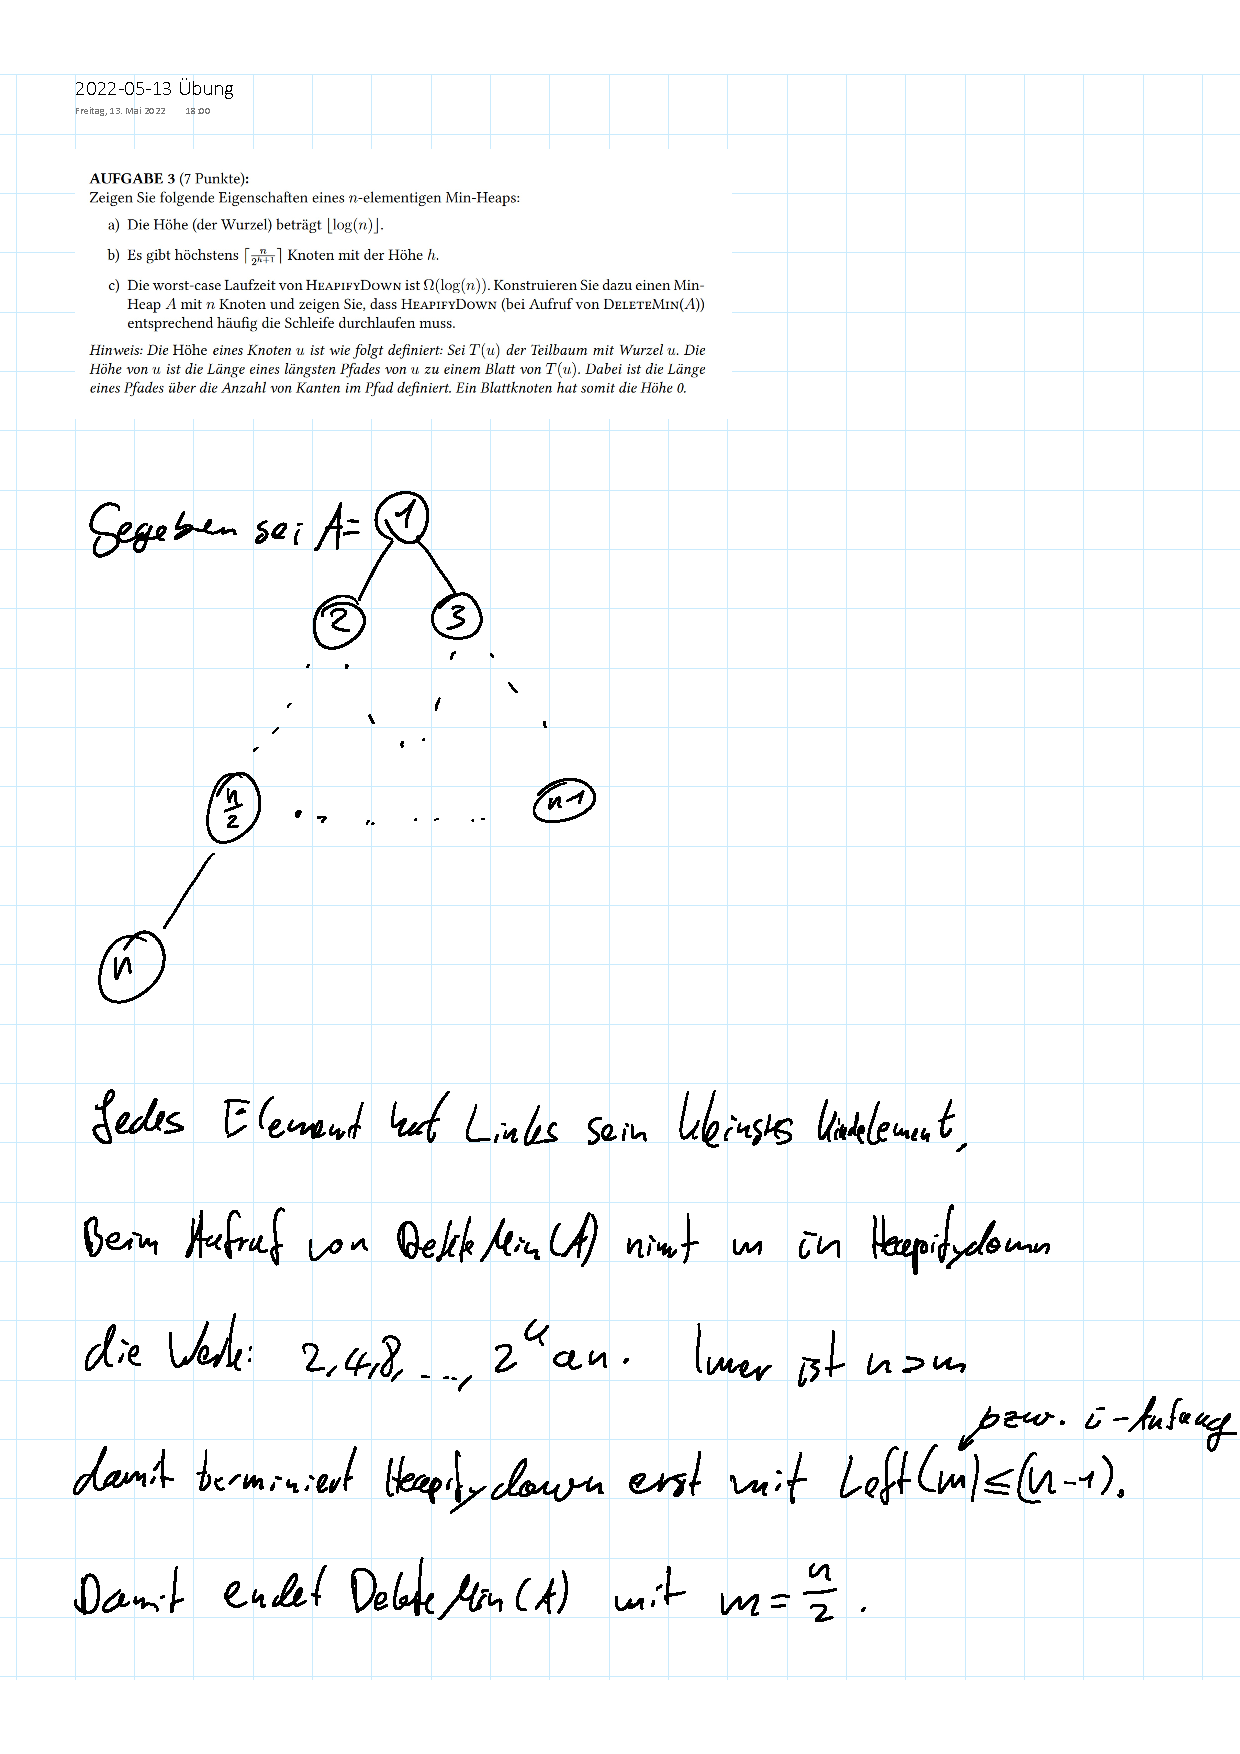
\includepdf[pages=-]{2022-05-13-DuA-beiProfGharibian-Heimblatt-05.pdf}

  \end{teilaufgabe}
\end{aufgabe}
\end{document}
